% algorithmes de plus courts chemins 

\begin{frame}{Graphes pondérés}

\begin{definition}
    Un graphe \emph{non-orienté pondéré} est un graphe non-orienté muni d'une fonction de pondération qui associe une valeur réelle à chaque arête. 
\end{definition}

\begin{definition}
    Un graphe \emph{orienté pondéré} est un graphe orienté muni d'une fonction de pondération qui associe une valeur réelle à chaque arc. 
\end{definition}

\end{frame}

\begin{frame}{Exemple : graphe non-orienté pondéré}
    \begin{center}
        \begin{tikzpicture}
\clip (0,0) rectangle (6,6);
\Vertex[x=0.450,y=5.550,size=0.8,opacity=0.5,label=1]{0}
\Vertex[x=0.450,y=3.000,size=0.8,opacity=0.5,label=2]{1}
\Vertex[x=3.000,y=3.000,size=0.8,opacity=0.5,label=3]{2}
\Vertex[x=3.000,y=5.550,size=0.8,opacity=0.5,label=4]{3}
\Vertex[x=5.550,y=5.550,size=0.8,opacity=0.5,label=5]{4}
\Vertex[x=5.550,y=3.000,size=0.8,opacity=0.5,label=6]{5}
\Vertex[x=5.550,y=0.450,size=0.8,opacity=0.5,label=7]{6}
\Vertex[x=3.000,y=0.450,size=0.8,opacity=0.5,label=8]{7}
\Vertex[x=0.450,y=0.450,size=0.8,opacity=0.5,label=9]{8}
\Edge[,lw=2.0,bend=-8.531,label=5](0)(1)
\Edge[,lw=2.0,bend=-8.531,label=2](0)(3)
\Edge[,lw=2.0,bend=-8.531,label=-2](1)(3)
\Edge[,lw=2.0,bend=-8.531,label=4](2)(8)
\Edge[,lw=2.0,bend=-8.531,label=1](4)(5)
\Edge[,lw=2.0,bend=-8.531,label=3](5)(6)
\Edge[,lw=2.0,bend=-8.531,label=0](6)(7)
\end{tikzpicture}

    \end{center}
    \end{frame}

% TODO exemple de graphe orienté avec pondération ?

\begin{frame}{Applications}
    \begin{itemize}
        \item Calcul de plus courts chemins 
        \begin{itemize}
            \item Distances entre villes
        \end{itemize}
        \item Arbres couvrants minimaux 
        \item Contraintes entre tâches 
    \end{itemize}
\end{frame}

\begin{frame}{Arbre couvrant}
    \begin{definition}
        Dans un graphe $G$ non orienté (pondéré ou non) connexe, un arbre couvrant est un sous-graphe connexe acyclique (arbre) incluant tous les sommets de $G$
    \end{definition}


\end{frame}

% TODO ajouter définition d'un sous-graphe 


\begin{frame}{Exemple : arbre couvrant}
    \begin{center}
        \begin{tikzpicture}
\clip (0,0) rectangle (6,6);
\Vertex[x=0.450,y=5.550,size=0.8,opacity=0.5,label=1]{0}
\Vertex[x=0.450,y=3.000,size=0.8,opacity=0.5,label=2]{1}
\Vertex[x=3.000,y=3.000,size=0.8,opacity=0.5,label=3]{2}
\Vertex[x=3.000,y=5.550,size=0.8,opacity=0.5,label=4]{3}
\Vertex[x=5.550,y=5.550,size=0.8,opacity=0.5,label=5]{4}
\Vertex[x=5.550,y=3.000,size=0.8,opacity=0.5,label=6]{5}
\Vertex[x=5.550,y=0.450,size=0.8,opacity=0.5,label=7]{6}
\Vertex[x=3.000,y=0.450,size=0.8,opacity=0.5,label=8]{7}
\Vertex[x=0.450,y=0.450,size=0.8,opacity=0.5,label=9]{8}
\Edge[,lw=2.0,bend=-8.531](0)(1)
\Edge[,lw=4.0,bend=-8.531](0)(3)
\Edge[,lw=4.0,bend=-8.531,](1)(3)
\Edge[,lw=4.0,bend=-8.531](2)(8)
\Edge[,lw=4.0,bend=-8.531](4)(5)
\Edge[,lw=4.0,bend=-8.531](5)(6)
\Edge[,lw=4.0,bend=-8.531](6)(7)
\Edge[,lw=4.0,bend=-8.531](3)(4)
\Edge[,lw=4.0,bend=-8.531](2)(6)
\Edge[,lw=2.0,bend=-8.531](2)(1)
\end{tikzpicture}

    \end{center}
    \end{frame}

    \begin{frame}{Contre-exemple : arbre non couvrant}
        \begin{center}
            \begin{tikzpicture}
\clip (0,0) rectangle (6,6);
\Vertex[x=0.450,y=5.550,size=0.8,opacity=0.5,label=1]{0}
\Vertex[x=0.450,y=3.000,size=0.8,opacity=0.5,label=2]{1}
\Vertex[x=3.000,y=3.000,size=0.8,opacity=0.5,label=3]{2}
\Vertex[x=3.000,y=5.550,size=0.8,opacity=0.5,label=4]{3}
\Vertex[x=5.550,y=5.550,size=0.8,opacity=0.5,label=5]{4}
\Vertex[x=5.550,y=3.000,size=0.8,opacity=0.5,label=6]{5}
\Vertex[x=5.550,y=0.450,size=0.8,opacity=0.5,label=7]{6}
\Vertex[x=3.000,y=0.450,size=0.8,opacity=0.5,label=8]{7}
\Vertex[x=0.450,y=0.450,size=0.8,opacity=0.5,label=9]{8}
\Edge[,lw=2.0,bend=-8.531](0)(1)
\Edge[,lw=4.0,bend=-8.531](0)(3)
\Edge[,lw=4.0,bend=-8.531,](1)(3)
\Edge[,lw=4.0,bend=-8.531](2)(8)
\Edge[,lw=2.0,bend=-8.531](4)(5)
\Edge[,lw=4.0,bend=-8.531](5)(6)
\Edge[,lw=4.0,bend=-8.531](6)(7)
\Edge[,lw=4.0,bend=-8.531](3)(4)
\Edge[,lw=4.0,bend=-8.531](2)(6)
\Edge[,lw=2.0,bend=-8.531](2)(1)
\end{tikzpicture}

        \end{center}
        \end{frame}
    
\begin{frame}{Construction d'un arbre couvrant}
\begin{itemize}
    \item Connaissez-vous un algorithme capable de construire un arbre couvrant ?
    \pause \item Oui !
    \pause \item Tous les algorithmes de parcours que nous avons vus jusqu'ici 
    \pause \item Pour de bonnes raisons applicatives, on va chercher à construire un arbre couvrant \emph{minimal} 
\end{itemize}
    
\end{frame}

\begin{frame}{Arbre couvrant minimal}
    \begin{definition}
        Dans un graphe non orienté pondéré et connexe, un arbre couvrant minimal est un arbre couvrant dont la somme des arêtes est minimale
    \end{definition}

    \begin{itemize}
        \item Remarque : si le graphe n'est pas pondéré, on considère des arêtes de poids identique 
    \end{itemize}
\end{frame}

\begin{frame}{Exemple 1 : arbre couvrant minimal (non pondéré)}
    \begin{center}
        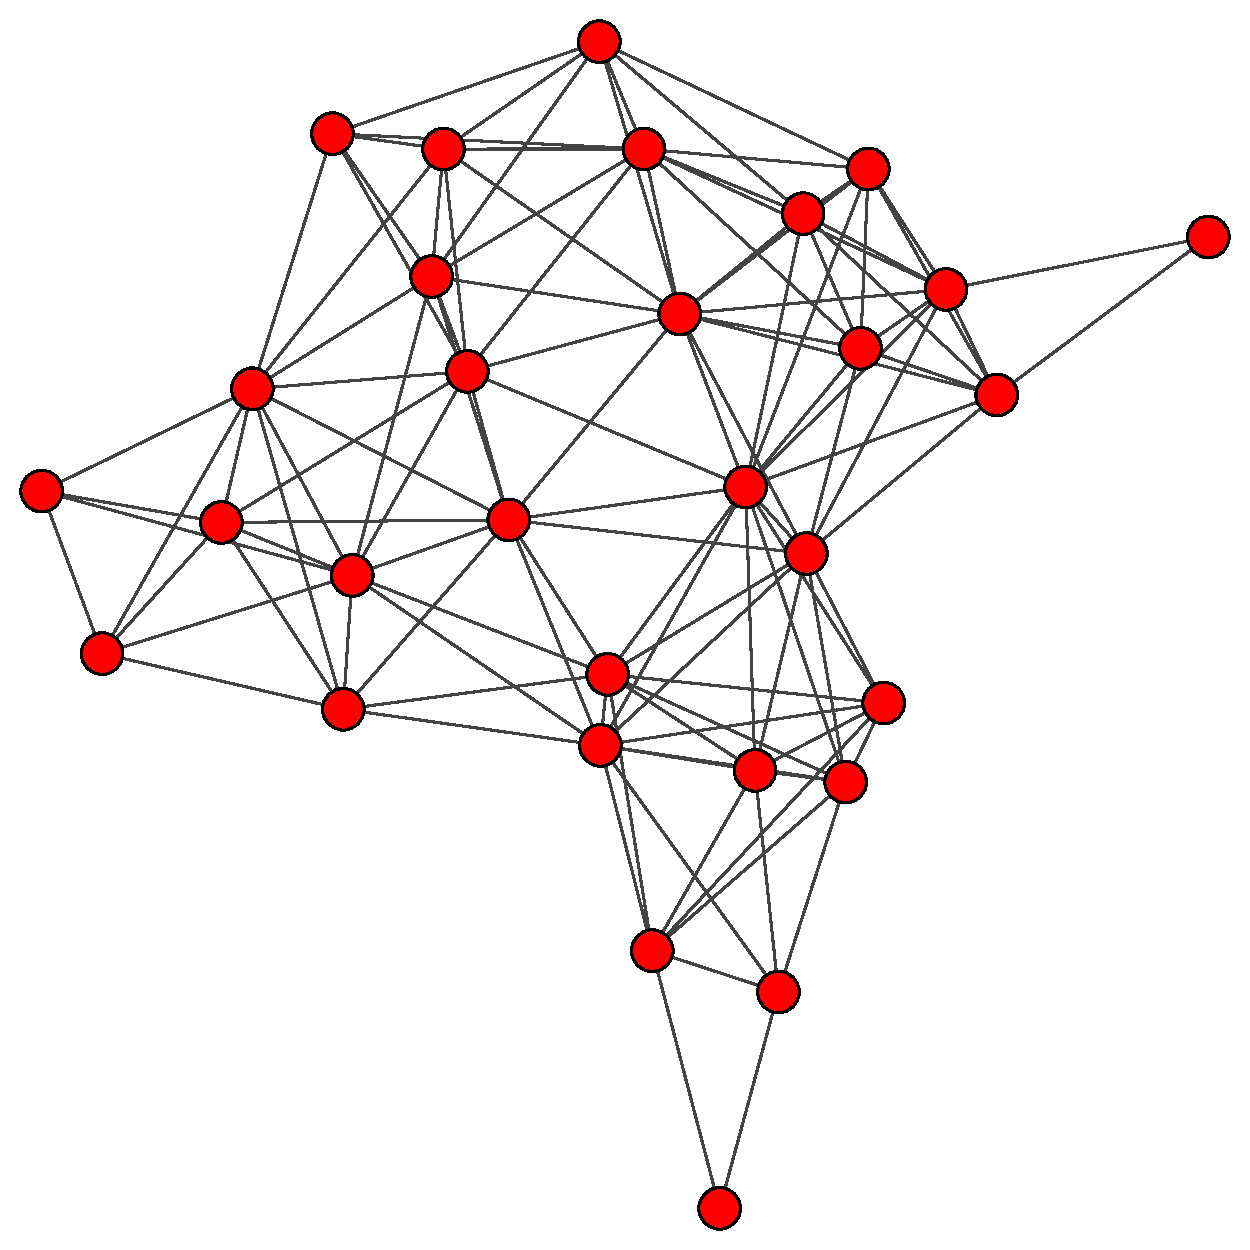
\includegraphics[height=.8\textheight]{fig/mst-0.pdf}
    \end{center}
\end{frame}
\begin{frame}{Exemple 1 : arbre couvrant minimal (non pondéré)}
    \begin{center}
        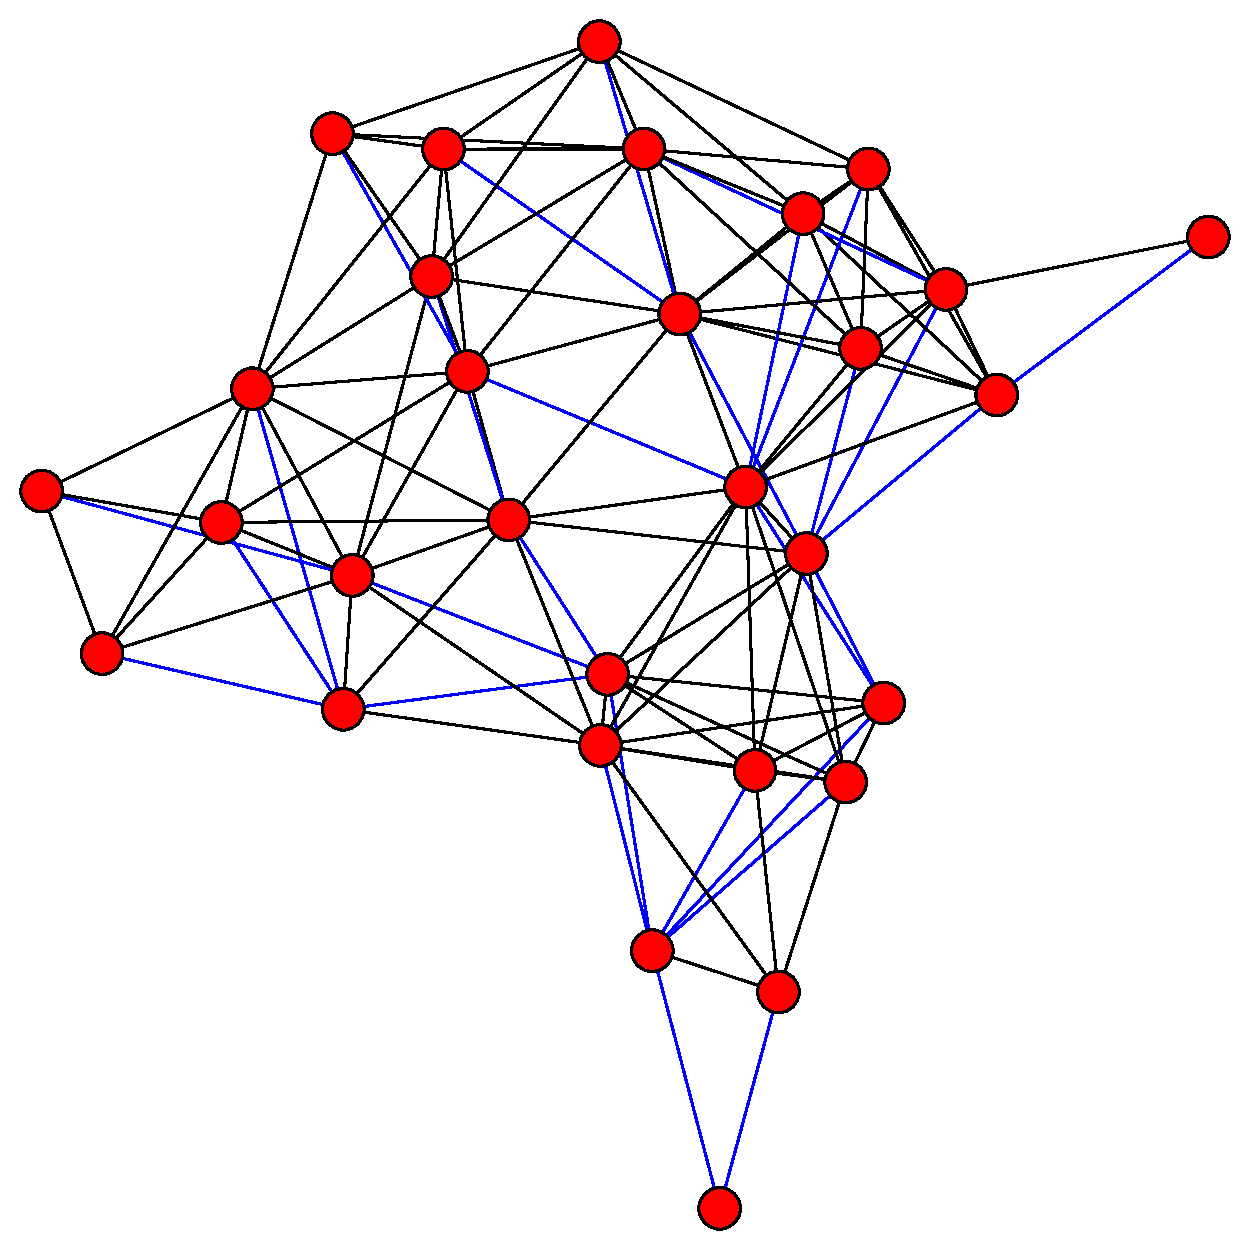
\includegraphics[height=.8\textheight]{fig/mst-1.pdf}
    \end{center}
\end{frame}
\begin{frame}{Exemple 1 : arbre couvrant minimal (non pondéré)}
    \begin{center}
        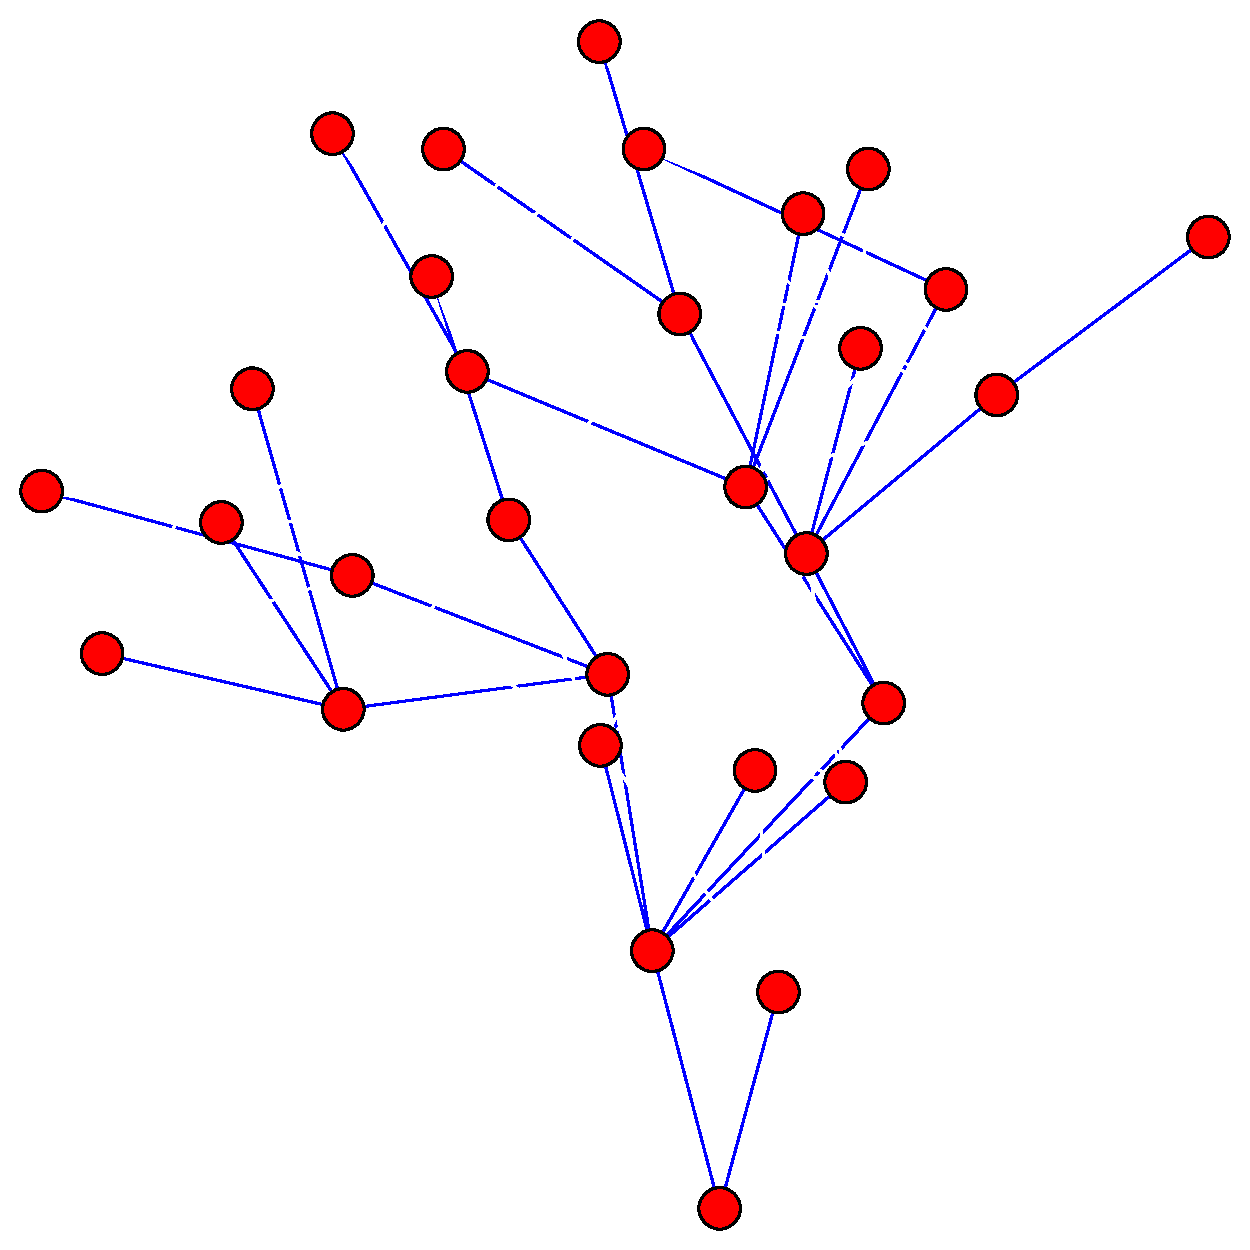
\includegraphics[height=.8\textheight]{fig/mst-2.pdf}
    \end{center}
\end{frame}

\begin{frame}{Exemple 2 : arbre couvrant minimal (pondéré)}
    \begin{center}
        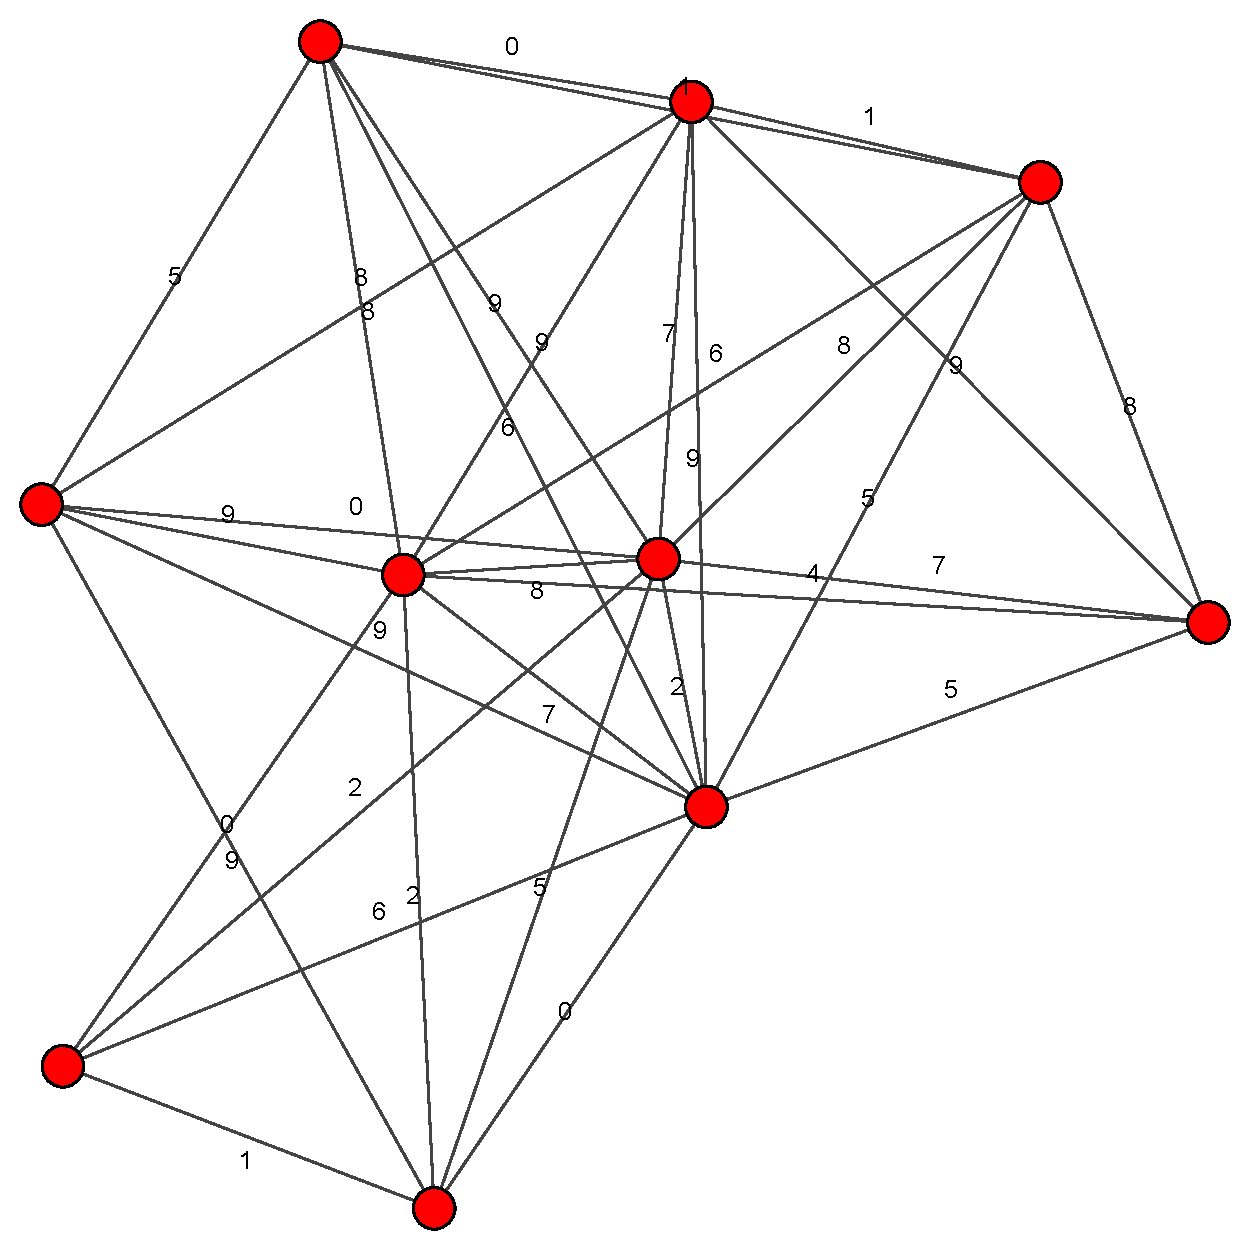
\includegraphics[height=.8\textheight]{fig/mstp-0.pdf}
    \end{center}
\end{frame}
\begin{frame}{Exemple 2 : arbre couvrant minimal (non pondéré)}
    \begin{center}
        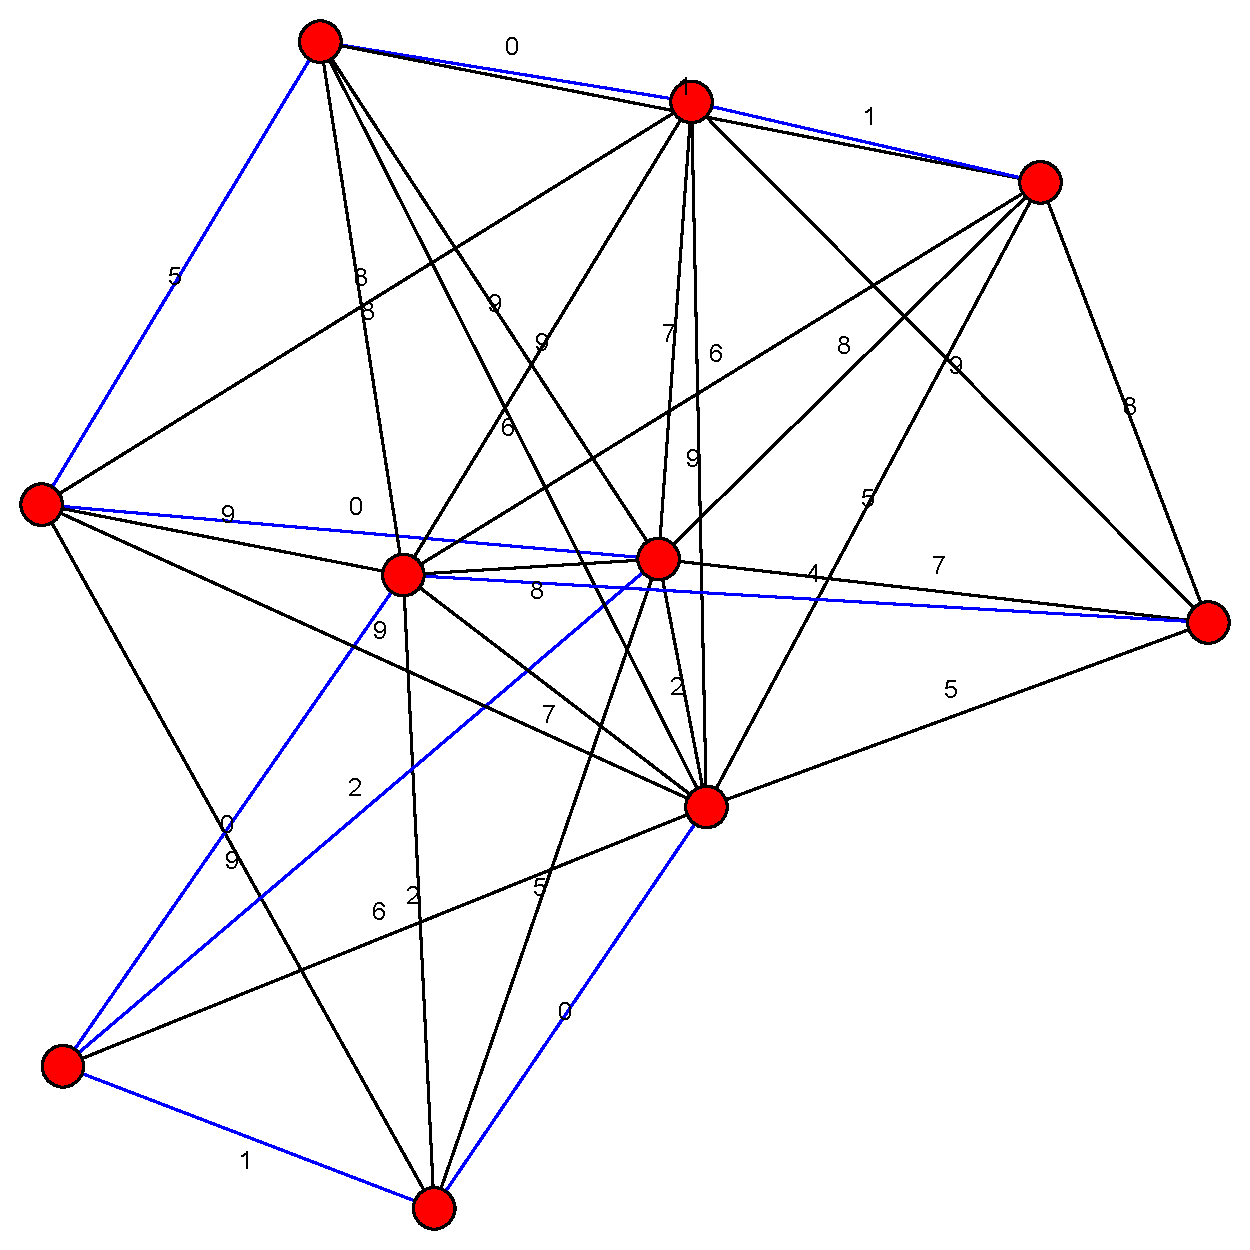
\includegraphics[height=.8\textheight]{fig/mstp-1.pdf}
    \end{center}
\end{frame}

% TODO algorithme glouton 

% TODO algorithme de Prim 

